% SVN info for this file
\svnidlong
{$HeadURL$}
{$LastChangedDate$}
{$LastChangedRevision$}
{$LastChangedBy$}

\chapter{BMI Internals}
\labelChapter{Chapter_3}

\begin{introduction}
  This chapter will describe some of the internals of how BMI works.
\end{introduction}

% to create and index select MakeIndex -> Run arrow, and then switch to pdfLaTeX and Run Arrow

\section{The Clone-Snapshot Workflow}

Central to the \index{BMI methodology}BMI methodology - especially with a Ceph networked-storage cluster, servicing images via a \index{RADOS Block Device (RBD)}\emph{RADOS Block Device (RBD)} - is the \index{Clone-Snapshot workflow}\emph{Clone-Snapshot} workflow: \\

\begin{figure}[!h] % Example of including images
\label{fig:bmi-workflow-import}
\begin{center}
%\includegraphics[width=0.5\linewidth]{#1}
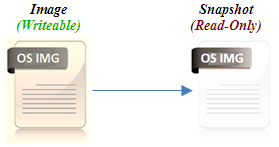
\includegraphics[scale=1]{figures/ceph-clone-snapshot.png}
\end{center}
\caption{The Clone-Snapshot Workflow}
%\label{fig:example_figure}
\end{figure}


Images are files used to iPXE boot from, which can also be written to.  Images \underline{\emph{cannot}} be cloned, though if one creates a snapshot - which is a point-in-time, read-only copy of an image that preserves its state - one can \index{clone}clone that \index{snapshot}snapshot to create a new child image.  These child images are now connected to the parent snapshot, but one can \index{flatten}\emph{flatten} them in order to copy over any dependent data to sever this connection, and thus make them independent. Therefore in order to ensure provenance, and also be able to extend the BMI workflow through new customized images, one always will create a snapshot after creating or cloning/flattening a new image.  By guaranteeing that all images will have a snapshot, one will always be able to connect to any image's snapshot to inherit and extend its state cloning.  All snapshots associated with images that are created through BMI are named \code{snapshot}. \\


The general overview connection between Ceph, RADOS, snapshots and images is illustrated in Figure \ref{fig:ceph_rados_snapshot_clone}\footnote{\link{https://www.packtpub.com/books/content/working-ceph-block-device}}. \\


\begin{figure}[!h] % Example of including images
\label{fig:bmi-workflow-import}
\begin{center}
%\includegraphics[width=0.5\linewidth]{#1}
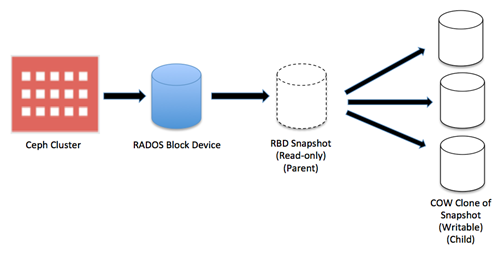
\includegraphics[scale=1]{figures/ceph-rados-snapshot-clone.png}
\end{center}
\caption{A Ceph cluster servicing a RADOS block device providing access to snapshots and images}
\label{fig:ceph_rados_snapshot_clone}
\end{figure}


\section{Importing an Image}

The concept behind importing an image into BMI is to create a duplicate of the image - considered the \index{Golden Image}\emph{Golden Image} in Ceph - so that we have a golden image from BMI's perspective to extend from.  The database column in BMI called \code{Ceph} contains the images associated with that instance of BMI, that are stored in Ceph.  Now any subsequent operation on a row in the \code{Name} column from the BMI database --- such as \emph{provisioning} or \emph{snapshotting} --- will actually clone the image's snapshot indicated in the \code{Ceph} column for that respective row of that name, and then create a snapshot as well. \\

The one difference when importing an image into BMI, is that there might not be a snapshot in the original image in Ceph.  For that reason, every time an image is imported into BMI, a snapshot is taken.  Afterwards a \index{clone-and-flatten}\emph{clone-and-flatten} operation is performed with a subsequent snapshot.  Since the flattening step makes the child image independent, BMI will remove the parent snapshot in order to save space.  In Figure \ref{fig:bmi-workflow-import}, the steps described above illustrate this workflow: \\ 


\begin{figure}[!h] % Example of including images
\label{fig:bmi-workflow-import}
\begin{center}
%\includegraphics[width=0.5\linewidth]{#1}
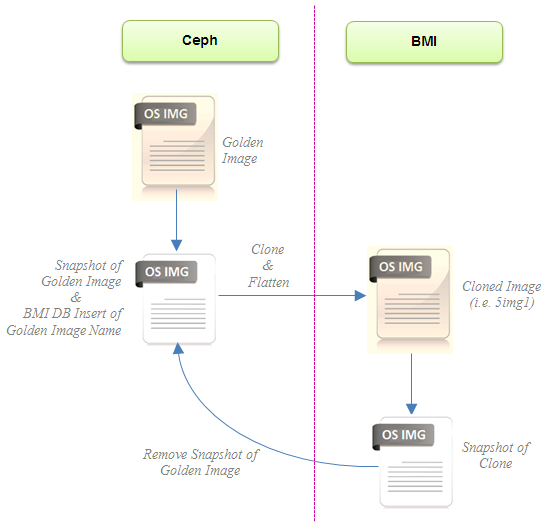
\includegraphics[scale=1]{figures/workflow-bmi-import-v2.png}
\end{center}
\caption{BMI Import Workflow}
%\label{fig:example_figure}
\end{figure}

\pagebreak

The steps that take place when importing and image into BMI are described in the following lines of code:

\begin{center}
\link{https://github.com/CCI-MOC/ims/blob/dev/ims/einstein/operations.py\#L431-L454}
\end{center}


\subsection{\index{Ceph image database name format}Ceph Image Name Format In The BMI Database}

One thing to mention, is that any image entry into the database under the \code{Ceph} column will be formatted using the following nomenclature: 

\begin{center}
\emph{\color{gray}PREFIX}\code{img}\emph{\color{gray}SUFFIX} 
\end{center}

The \code{PREFIX} is configured via the \code{/etc/bmi/bmiconfig.cfg} file, through the \code{uid} variable --- available under the \code{[bmi]} heading:

\code{
\text{} \\
\text{}\hspace{6mm} [bmi] \\
\text{}\hspace{6mm} uid = 5 \\
}

The \code{SUFFIX} begin with 1 and will continue to increment with every new addition to the database.  The same value will also stored under the \code{Id} column.

